\documentclass[aspectratio=169,10pt]{beamer}

\usetheme{Madrid}
\usecolortheme{default}
\setbeamertemplate{navigation symbols}{}
\setbeamertemplate{footline}[frame number]
\setbeamertemplate{frametitle}{
  \nointerlineskip
  \begin{beamercolorbox}[wd=\paperwidth,ht=2.8ex,dp=1.2ex,leftskip=1em]{frametitle}
    \usebeamerfont{frametitle}May 10, 2026 -- \insertframetitle
  \end{beamercolorbox}
}

\usepackage[T1]{fontenc}
\usepackage{lmodern}
\usepackage{amsmath,amssymb,bm}
\usepackage{booktabs}
\usepackage{tabularx}
\usepackage{listings}
\usepackage{xcolor}
\usepackage{hyperref}
\usepackage{tikz}
\usetikzlibrary{positioning}

\definecolor{singlepink}{RGB}{150,35,65}
\definecolor{singlebg}{RGB}{255,239,244}
\definecolor{codebg}{RGB}{248,248,248}
\definecolor{codeframe}{RGB}{210,210,210}
\definecolor{codekw}{RGB}{20,65,140}
\definecolor{softgreen}{RGB}{230,248,236}
\definecolor{softorange}{RGB}{255,244,224}
\definecolor{softblue}{RGB}{226,239,255}

\lstdefinestyle{codesmall}{
  basicstyle=\ttfamily\fontsize{6.0}{6.6}\selectfont,
  keywordstyle=\color{codekw},
  commentstyle=\color{gray},
  stringstyle=\color{singlepink},
  showstringspaces=false,
  breaklines=true,
  columns=fullflexible,
  keepspaces=true,
  frame=single,
  framerule=0.3pt,
  backgroundcolor=\color{codebg},
  rulecolor=\color{codeframe},
  tabsize=4
}

\newcommand{\code}[1]{\ifmmode\text{\ttfamily\detokenize{#1}}\else\texttt{\detokenize{#1}}\fi}
\newcommand{\pathsmall}[1]{{\scriptsize\path{#1}}}
\newcommand{\fileanchor}[2]{{\scriptsize\color{gray}\textbf{Code anchor:} \path{#1}; \code{#2}\par}}
\newcommand{\important}[1]{\begin{block}{Key point}\small #1\end{block}}
\newcommand{\proposal}[1]{\begin{beamercolorbox}[rounded=true,wd=\textwidth,sep=0.8em]{block body}\small #1\end{beamercolorbox}}
\newcommand{\dd}{\,\mathrm d}

\title[Godlog May 10, 2026]{Godlog - May 10, 2026\\Single-Detector LLR/FAR Proposal for SPIIR}
\subtitle{Local implementation plan for the Eric branch}
\author{SPIIR workflow notes}
\date{May 10, 2026}

\begin{document}

\begin{frame}{Godlog}
\titlepage
\end{frame}

\begin{frame}{Purpose of This Godlog}
\small
This file records the proposed single-detector implementation for the Eric branch.
The intent is:
\begin{itemize}
  \item use the main SPIIR pipeline as the stable upstream coherent search;
  \item use the \code{wguo-single-detector} branch as the baseline for single-detector row extraction/routing;
  \item add the missing piece: a single-detector likelihood-ratio rank and FAR assignment path;
  \item keep the proposal focused on the single branch only.
\end{itemize}

\important{
The final single-detector target is not a raw \((\rho_m,\chi_r^2)\) plot.  The target calibrated product is
\[
(\rho_m,-\log_{10}\mathrm{FAR}_{\mathrm{sd}}).
\]
}
\end{frame}

\begin{frame}{Code Bases to Combine in the Eric Branch}
\small
\begin{tabularx}{\textwidth}{p{0.22\textwidth}X}
\toprule
Source & Role in the realization \\
\hline
Main SPIIR & Provides the online/offline postcoh pipeline, detector conditioning, SPIIR filtering, \code{cuda_postcoh}, coherent background/FAR, and \code{FinalSink}. \\
\code{wguo-single-detector} & Provides the single-detector extraction idea: preserve detector-local information from postcoh/coexistence rows so H1 and L1 can be analyzed as independent single-detector categories. \\
Eric branch & Should combine the two bases and add the new single-detector LLR/FAR layer described here. \\
\bottomrule
\end{tabularx}

\vspace{0.7em}
\pathsmall{https://git.ligo.org/lscsoft/spiir}

\pathsmall{https://git.ligo.org/lscsoft/spiir/-/tree/wguo-single-detector?ref_type=heads}

\vspace{0.8em}
The local code in this workspace is not a Git checkout, so the changes are prepared locally for later push by the user.
\end{frame}

\begin{frame}{What Already Exists}
\small
\begin{columns}[T,onlytextwidth]
\column{0.49\textwidth}
\textbf{Upstream products already available}
\begin{itemize}
  \item detector-local complex SNR streams;
  \item local peak SNR amplitudes \(\code{snglsnr[j]}\);
  \item detector-local autochisq values \(\code{chisq[j]}\);
  \item row flags: foreground, background, empty;
  \item bank/template/time metadata;
  \item coherent quantities such as \(\code{cohsnr}\), \(\code{nullsnr}\), and \(\code{cmbchisq}\).
\end{itemize}

\column{0.49\textwidth}
\textbf{Single-side interpretation}
\[
\rho_m=\code{snglsnr[j]},
\qquad
\chi_r^2=\code{chisq[j]}.
\]

For each detector \(j\in\{\mathrm{H1},\mathrm{L1}\}\), one postcoh row can produce a detector-local feature
\[
d_{j,m}=(\rho_m,\chi_r^2).
\]
\end{columns}
\end{frame}

\begin{frame}{What Is Missing}
\small
The current code can expose the needed observables, but the single branch still needs a complete statistical significance layer:
\begin{enumerate}
  \item define \(H_0\) and \(H_1\) likelihoods for \((\rho_m,\chi_r^2)\);
  \item compute a log-likelihood-ratio rank \(r(d)\);
  \item accumulate a single-detector rank background;
  \item persist that background in a dedicated single FAR--LLR file;
  \item assign FAR from the rank-tail count and livetime;
  \item output \((\rho_m,-\log_{10}\mathrm{FAR}_{\mathrm{sd}})\) rows.
\end{enumerate}

\proposal{
The single-detector background file is only a FAR--LLR/rank-livetime file.  It is not the coherent XML statistics file and it is not a persistent two-dimensional \((\rho_m,\chi_r^2)\) map.
}
\end{frame}

\begin{frame}{Single-Branch Boundary in the Pipeline}
\small
\fileanchor{spiir/gstlal-spiir/python/pipemodules/spiirparts.py}{mkPostcohSPIIROnline(...), after mkcudapostcoh(...)}

The natural branch point is after \code{cuda_postcoh}, because this is the first point where every postcoh row already contains:
\[
\code{snglsnr[j]},\quad \code{chisq[j]},\quad
\code{is_background},\quad \code{ifos},\quad \code{tmplt_idx},\quad \code{bankid}.
\]

\begin{center}
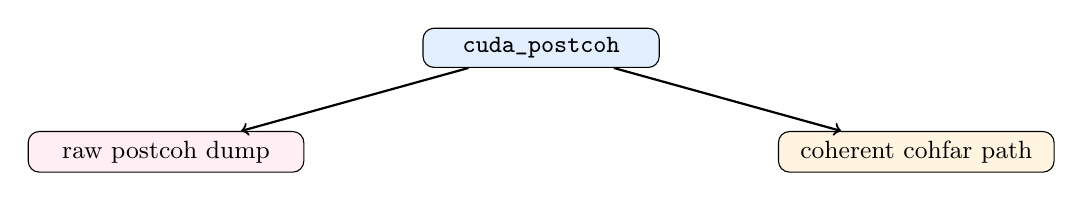
\begin{tikzpicture}[node distance=1.1cm, every node/.style={font=\small}]
\node[draw, rounded corners, fill=softblue, minimum width=3.0cm] (post) {\code{cuda_postcoh}};
\node[draw, rounded corners, fill=singlebg, below left=0.8cm and 1.5cm of post, minimum width=3.5cm] (single) {raw postcoh dump};
\node[draw, rounded corners, fill=softorange, below right=0.8cm and 1.5cm of post, minimum width=3.5cm] (coh) {coherent cohfar path};
\draw[->, thick] (post) -- (single);
\draw[->, thick] (post) -- (coh);
\end{tikzpicture}
\end{center}

The single branch must not recompute matched filtering, \(C_{j,m}\), \(\code{cohsnr}\), or \(\code{cmbchisq}\).  It reuses the detector-local pair already created upstream.
\end{frame}

\begin{frame}[fragile]{Current Local Hook in \code{pipeline.sh}}
\small
\fileanchor{spiir/pipeline.sh}{mode parser and post-graph single analyzer call}

\begin{lstlisting}[style=codesmall,language=bash]
PIPELINE_MODE="${PIPELINE_MODE:-}"
...
export PIPELINE_MODE
"${base_cmd[@]}"

single_far_csv="${jobno}/${jobno}_single_detector_far.csv"
single_far_background_input="${SINGLE_FAR_BACKGROUND_INPUT:-}"
single_far_background_output="${SINGLE_FAR_BACKGROUND_OUTPUT:-${jobno}/${jobno}_single_far_llr_background.json}"
\end{lstlisting}

\vspace{0.4em}
In \code{--single} mode, the coherent GStreamer graph still runs.  After that graph exits, the offline single analyzer reads \code{sdpostcoh*.xml.gz} and writes single-detector FAR rows.
\end{frame}

\begin{frame}[fragile]{Local Code Added to Launch LLR/FAR}
\small
\fileanchor{spiir/pipeline.sh}{single_detector_cmd}

\begin{lstlisting}[style=codesmall,language=bash]
single_detector_cmd=(
  python "${single_detector_py}" single
  --postcoh-glob "${jobno}/sdpostcoh*.xml.gz"
  --output "${single_far_csv}"
  --ifos H1,L1
  --min-snr 4
  --background-output "${single_far_background_output}"
  --snr-bins "${SINGLE_FAR_SNR_BINS:-4,6,8,12,inf}"
)
if [[ -n "${single_far_background_input}" ]]; then
  single_detector_cmd+=(--background-input "${single_far_background_input}")
fi
if [[ "${single_far_calibrate}" == "1" ]]; then
  single_detector_cmd+=(--calibrate-noise-dof)
fi
"${single_detector_cmd[@]}"
\end{lstlisting}

\proposal{
Cold start: if no \code{SINGLE_FAR_BACKGROUND_INPUT} is supplied, the run calibrates from the current background rows and writes the first \code{single_far_llr_background.json}.  Later runs load that file and update it.
}
\end{frame}

\begin{frame}{Single-Detector Categories}
\small
The single branch only uses detector-local H1 and L1 information:
\[
j\in\{\mathrm{H1},\mathrm{L1}\}.
\]
They are analyzed separately, not as a coherent HL network:
\[
\mathrm{H1}\to \mathrm{H1\_sd},
\qquad
\mathrm{L1}\to \mathrm{L1\_sd}.
\]

For each available detector,
\[
\rho_m=\code{snglsnr[j]},\qquad \chi_r^2=\code{chisq[j]}.
\]

\important{
If only H1 or only L1 is available because the other detector loses lock, the available detector can still contribute to its own single-detector category.
}
\end{frame}

\begin{frame}{Coexistence Rows and the wguo Extraction Idea}
\small
A multi-detector coexistence row, for example HL or HLV, can still carry detector-local fields:
\[
\code{snglsnr[H1]},\quad \code{chisq[H1]},\quad
\code{snglsnr[L1]},\quad \code{chisq[L1]}.
\]

The single branch should copy the detector-local H1/L1 pairs into the single categories:
\[
\mathrm{H1}: (\code{snglsnr[H1]},\code{chisq[H1]})\to \mathrm{H1\_sd},
\]
\[
\mathrm{L1}: (\code{snglsnr[L1]},\code{chisq[L1]})\to \mathrm{L1\_sd}.
\]

This is not numerical subtraction.  The coherent row remains in the coherent branch; the single branch only duplicates the local H/L pair for independent single-detector ranking.
\end{frame}

\begin{frame}{Feature Extraction From Postcoh Rows}
\small
\fileanchor{spiir/gstlal-spiir/python/pipemodules/single_detector_far.py}{features_from_postcoh_row}

For every postcoh row and every requested detector \(j\), the analyzer reads:
\[
\rho_m=\code{snglsnr[j]},
\qquad
\chi_r^2=\code{chisq[j]}.
\]
It rejects missing, nonpositive, or below-threshold values.  The retained object is:
\[
d_{j,m}=(\rho_m,\chi_r^2).
\]

\proposal{
The single branch does not inspect the full SNR stream at this stage.  It trusts \code{cuda_postcoh} to have already selected the trigger peak and computed the detector-local autochisq around that peak.
}
\end{frame}

\begin{frame}{Meaning of \(\rho_m\)}
\small
For fixed detector \(j\) and template \(m\), SPIIR has a complex SNR time series:
\[
\rho_{j,m}(t).
\]
A trigger is centered at one detector-local peak time \(t_j\).  The complex peak value is
\[
\hat\rho_{j,m}=\rho_{j,m}(t_j).
\]
The single-detector SNR coordinate is the peak amplitude:
\[
\rho_m=|\hat\rho_{j,m}|=\code{snglsnr[j]}.
\]

\important{
\(\rho_m\) is the peak SNR for this detector and this template.  It is not \(\code{cohsnr}\), because no network projection is used in the single branch.
}
\end{frame}

\begin{frame}{Meaning of \(\chi_r^2\)}
\small
The detector-local shape statistic compares the SNR samples around the peak to the stored local template shape:
\[
r_{j,m}(\Delta)=
\rho_{j,m}(t_j+\Delta)-\hat\rho_{j,m}C_{j,m}(\Delta),
\qquad \Delta=-L,\ldots,L.
\]
The reduced statistic is
\[
\chi_r^2\equiv\chi_{j,m}^2
=
\frac{1}{N_{j,m}}
\sum_{\Delta=-L}^{L}|r_{j,m}(\Delta)|^2.
\]

In code this is stored as:
\[
\chi_r^2=\code{chisq[j]}.
\]
Small \(\chi_r^2\) means the local window is consistent with the template shape; large \(\chi_r^2\) is more glitch-like.
\end{frame}

\begin{frame}{Likelihood Hypotheses}
\small
The new rank uses two statistical hypotheses:
\begin{description}
  \item[\(H_0\)] noise/glitch hypothesis: the local peak is noise-like.  The residual shape has no deterministic signal-like shift.
  \item[\(H_1\)] signal hypothesis: the local peak is signal-like.  The residual may contain Gaussian noise plus a small deterministic template-mismatch shift.
\end{description}

The desired rank is a log-likelihood ratio:
\[
r(d)\simeq
\ln\frac{P(d\mid H_1)}{P(d\mid H_0)},
\qquad d=(\rho_m,\chi_r^2).
\]

Using the product rule:
\[
r(d)=
\ln\frac{P(\chi_r^2\mid\rho_m,H_1)}
        {P(\chi_r^2\mid\rho_m,H_0)}
+
\ln\frac{P(\rho_m\mid H_1)}{P(\rho_m\mid H_0)}
+\mathrm{const}.
\]
\end{frame}

\begin{frame}{Why the Noise Side Is Chi-Square-Like}
\small
In the ideal exact-match case,
\[
\rho_{j,m}(t_j+\Delta)=\hat\rho_{j,m}C_{j,m}(\Delta)+n(\Delta),
\]
so the residual is
\[
r_{j,m}(\Delta)=n(\Delta).
\]
After whitening, the local noise is modeled as Gaussian in the complex components.  Therefore
\[
|r_{j,m}(\Delta)|^2
=r_{\mathrm{re}}(\Delta)^2+r_{\mathrm{im}}(\Delta)^2
\]
is a sum of Gaussian squares, and the local quadratic power is chi-square-like.

\proposal{
The actual online trigger stream is peak-selected and clustered, so the ideal degree count is not trusted directly.  We use an empirical effective degree of freedom \(\nu_{\mathrm{eff}}\).
}
\end{frame}

\begin{frame}{Noise-Side Likelihood}
\small
Under \(H_0\), there is no deterministic mismatch shift:
\[
\lambda=0.
\]
The working model is a reduced central chi-square:
\[
Y=\nu_{\mathrm{eff}}\chi_r^2,
\qquad
Y\mid H_0\sim \chi^2_{\nu_{\mathrm{eff}}}.
\]
Therefore the density for the observed reduced statistic is
\[
P(\chi_r^2\mid\rho_m,H_0)
=
\nu_{\mathrm{eff}}
f_{\chi^2_{\nu_{\mathrm{eff}}}}
\bigl(\nu_{\mathrm{eff}}\chi_r^2\bigr).
\]

\important{
\(\nu_{\mathrm{eff}}\) is not calculated from a single trigger.  It must be calibrated from many background/noise triggers in the same category, optionally in SNR bins.
}
\end{frame}

\begin{frame}{Calibrating \(\nu_{\mathrm{eff}}\)}
\small
For a background category, such as \(\mathrm{H1\_sd}\), collect background triggers and read:
\[
\chi_{r,k}^2=\code{chisq[j]},\qquad k=1,\ldots,N_{\mathrm{bg}}.
\]
If the reduced statistic follows
\[
\chi_r^2\sim \frac{1}{\nu_{\mathrm{eff}}}\chi^2_{\nu_{\mathrm{eff}}},
\]
then
\[
\mathrm{Var}(\chi_r^2)=\frac{2}{\nu_{\mathrm{eff}}}.
\]
So a simple calibration is
\[
\nu_{\mathrm{eff}}\approx
\frac{2}{\mathrm{Var}_{\mathrm{bg}}(\chi_r^2)}.
\]

The local code now supports SNR-bin calibration:
\[
\rho_m\in[4,6),[6,8),[8,12),[12,\infty).
\]
\end{frame}

\begin{frame}{Signal-Side Mismatch Model}
\small
Under \(H_1\), a real signal may not perfectly match the stored local template shape.  Write
\[
s_{j,m}(\Delta)=
\hat\rho_{j,m}C_{j,m}(\Delta)\bigl(1+\beta(\Delta)\bigr).
\]
Then the tested residual becomes
\[
r_{j,m}(\Delta)
=
n(\Delta)+\beta(\Delta)\hat\rho_{j,m}C_{j,m}(\Delta).
\]
Within the short local window, approximate
\[
\beta(\Delta)\approx\bar\beta.
\]

\important{
The residual is Gaussian noise plus a deterministic mismatch shift.  This is why the signal-side shape likelihood is modeled with a noncentral chi-square distribution.
}
\end{frame}

\begin{frame}{The Noncentrality Parameter \(\lambda\)}
\small
Define the deterministic mismatch shift
\[
\mu(\Delta)=\bar\beta\,\hat\rho_{j,m}C_{j,m}(\Delta).
\]
For a sum of squared Gaussian variables with deterministic mean shift, the noncentrality is the squared norm of that shift:
\[
\lambda=\sum_{\Delta=-L}^{L}|\mu(\Delta)|^2.
\]
Substituting \(\mu(\Delta)\) gives
\[
\lambda(\bar\beta,\rho_m)
=
\bar\beta^2\rho_m^2
\sum_{\Delta=-L}^{L}|C_{j,m}(\Delta)|^2.
\]

\proposal{
\(\lambda\) is not a new measured feature.  It is the noncentral chi-square parameter introduced by the likelihood model.  It grows with mismatch level, peak SNR, and local template-shape power.
}
\end{frame}

\begin{frame}{Signal-Side Likelihood}
\small
For fixed \(\bar\beta\), use
\[
Y=\nu_{\mathrm{eff}}\chi_r^2,
\qquad
Y\mid(\rho_m,\bar\beta,H_1)
\sim
\chi^2_{\nu_{\mathrm{eff}}}(\lambda).
\]
Thus
\[
P(\chi_r^2\mid\rho_m,\bar\beta,H_1)
=
\nu_{\mathrm{eff}}
f_{\chi^2_{\nu_{\mathrm{eff}}}(\lambda)}
\bigl(\nu_{\mathrm{eff}}\chi_r^2\bigr).
\]

Because the true \(\bar\beta\) is unknown event by event, treat it as a nuisance parameter:
\[
\bar\beta\sim\mathrm{Uniform}(0,\beta_{\max}).
\]
\end{frame}

\begin{frame}{Marginalized Signal Likelihood}
\small
The final signal-side likelihood averages over allowed mismatch levels:
\[
P(\chi_r^2\mid\rho_m,H_1)
=
\frac{1}{\beta_{\max}}
\int_{0}^{\beta_{\max}}
\nu_{\mathrm{eff}}
f_{\chi^2_{\nu_{\mathrm{eff}}}(\lambda(\bar\beta,\rho_m))}
\bigl(\nu_{\mathrm{eff}}\chi_r^2\bigr)
\dd\bar\beta.
\]

In the code this is evaluated by a discrete beta grid:
\[
P(\chi_r^2\mid\rho_m,H_1)
\approx
\sum_i w_i\,g_i(\chi_r^2;\rho_m,\beta_i),
\qquad
\sum_i w_i=1.
\]

\proposal{
The prototype default uses \(\beta_{\max}=0.03\) and a uniform beta grid.  The grid and weights are implementation choices that should later be calibrated or validated with injections/background.
}
\end{frame}

\begin{frame}{Full Single-Detector Rank}
\small
The full single-detector rank is
\[
r(d)
=
\ln\frac{
P(\chi_r^2\mid\rho_m,H_1)}
{P(\chi_r^2\mid\rho_m,H_0)}
+
\frac{1}{2}\rho_m^2
+\mathrm{const}.
\]

The term \(+\rho_m^2/2\) is the SNR-amplitude contribution from the matched-filter likelihood after maximizing over amplitude/phase/time.

\vspace{0.5em}
For ranking, any fixed prior odds only add a constant:
\[
\ln\frac{P(H_1\mid d)}{P(H_0\mid d)}
=r(d)+\ln\frac{P(H_1)}{P(H_0)}.
\]
Therefore \(r(d)\) is enough to order events.
\end{frame}

\begin{frame}[fragile]{Local Likelihood Implementation}
\small
\fileanchor{spiir/gstlal-spiir/python/pipemodules/single_detector_far.py}{SingleDetectorLikelihoodModel}

\begin{lstlisting}[style=codesmall,language=Python]
def log_signal_shape_pdf(self, rho, chisq, autocorr_power=None, ifo=None):
    dof = self.signal_dof_for(rho, ifo)
    x = dof * float(chisq)
    terms = []
    for beta, weight in zip(self.beta_grid, self.beta_weights):
        lam = self.noncentrality(rho, beta, autocorr_power)
        terms.append(math.log(weight) + noncentral_chisq_logpdf(
            x, dof, lam, max_terms=self.ncx2_max_terms))
    return math.log(dof) + logsumexp(terms)

def log_noise_shape_pdf(self, rho, chisq, ifo=None):
    dof = self.noise_dof_for(rho, ifo)
    x = dof * float(chisq)
    return math.log(dof) + central_chisq_logpdf(x, dof)
\end{lstlisting}

The factor \(\log(\nu_{\mathrm{eff}})\) is the Jacobian from \(Y=\nu_{\mathrm{eff}}\chi_r^2\).
\end{frame}

\begin{frame}[fragile]{Local Rank Implementation}
\small
\fileanchor{spiir/gstlal-spiir/python/pipemodules/single_detector_far.py}{log_likelihood_ratio and rank}

\begin{lstlisting}[style=codesmall,language=Python]
def log_likelihood_ratio(self, rho, chisq, autocorr_power=None, ifo=None):
    shape_llr = (
        self.log_signal_shape_pdf(rho, chisq, autocorr_power, ifo=ifo)
        - self.log_noise_shape_pdf(rho, chisq, ifo=ifo))
    snr_llr = self.snr_log_weight * float(rho) * float(rho)
    return shape_llr + snr_llr + self.rank_offset

def rank(self, rho, chisq, autocorr_power=None, ifo=None):
    return self.log_likelihood_ratio(rho, chisq, autocorr_power, ifo=ifo)
\end{lstlisting}

\proposal{
This turns every single-detector feature \(d=(\rho_m,\chi_r^2)\) into one scalar \(r\).  Larger \(r\) means more signal-like.
}
\end{frame}

\begin{frame}{Rank-Space Background}
\small
For every single-detector background trigger, compute
\[
r_k^{(\mathrm{bg})}=r(d_k^{(\mathrm{bg})}).
\]
For a foreground candidate with rank \(r_*\), count same-category background triggers with rank at least as large:
\[
N_{\mathrm{bg}}^{(j)}(\ge r_*)
=
\sum_{k=1}^{N_{\mathrm{bg}}^{(j)}}
\mathbf 1\!\left(r_k^{(\mathrm{bg},j)}\ge r_*\right).
\]
The indicator function is one if the condition is true and zero otherwise.

\important{
This is the single-detector replacement for the old two-dimensional coherent rank-map lookup.  The significance calculation is one-dimensional in \(r\).
}
\end{frame}

\begin{frame}{FAR From the Rank Tail}
\small
Let \(T_{\mathrm{bg}}^{(j)}\) be the background livetime for the same detector category.  The final single-detector FAR is
\[
\mathrm{FAR}^{(j)}_{\mathrm{sd}}(r_*)
=
\frac{N_{\mathrm{bg}}^{(j)}(\ge r_*)}
{T_{\mathrm{bg}}^{(j)}}.
\]
The final plotted coordinate is
\[
\bigl(\rho_m,-\log_{10}\mathrm{FAR}^{(j)}_{\mathrm{sd}}\bigr).
\]

\proposal{
H1 and L1 must keep separate background rank lists and separate livetimes before any final display/alert-level merge.
}
\end{frame}

\begin{frame}[fragile]{Local Background Accumulator}
\small
\fileanchor{spiir/gstlal-spiir/python/pipemodules/single_detector_far.py}{RankBackground}

\begin{lstlisting}[style=codesmall,language=Python]
class RankBackground(object):
    def __init__(self):
        self._ranks = []
        self.livetime = 0.0

    def add_rank(self, rank):
        bisect.insort(self._ranks, float(rank))

    def count_ge(self, rank):
        idx = bisect.bisect_left(self._ranks, float(rank))
        return len(self._ranks) - idx

    def far(self, rank):
        if self.livetime <= 0.0:
            return 0.0
        return self.count_ge(rank) / self.livetime
\end{lstlisting}

This exact sorted-list version is suitable for offline validation.  A production version can replace it with a compact histogram or quantile/rank summary if memory becomes too large.
\end{frame}

\begin{frame}{Single FAR--LLR Background File}
\small
\fileanchor{spiir/gstlal-spiir/python/pipemodules/single_detector_far.py}{SingleFarLlrBackgroundFile}

The single background file stores only what FAR assignment needs:
\begin{itemize}
  \item detector categories, e.g. \(\mathrm{H1\_sd}\), \(\mathrm{L1\_sd}\);
  \item background LLR/rank values \(r_k^{(\mathrm{bg},j)}\);
  \item category livetimes \(T_{\mathrm{bg}}^{(j)}\);
  \item the likelihood/calibration model used to compute those ranks.
\end{itemize}

\[
\mathcal B_j=
\left\{
r_1^{(\mathrm{bg},j)},\ldots,r_N^{(\mathrm{bg},j)};
T_{\mathrm{bg}}^{(j)};
\nu_{\mathrm{eff}}(\rho_m)
\right\}.
\]

\important{
This file is the single-detector FAR--LLR file.  It is not a coherent-style \code{cohfar} XML statistics file.
}
\end{frame}

\begin{frame}{Cold Start and Real-Time Update Logic}
\small
At the beginning, no single FAR--LLR background file exists.  The first stage is a bootstrap:
\begin{enumerate}
  \item run the single analyzer over about one week of data;
  \item collect background rows and empty-row livetime;
  \item calibrate \(\nu_{\mathrm{eff}}\) from background \(\chi_r^2\);
  \item compute ranks for background and foreground rows;
  \item assign provisional FAR from the in-run background;
  \item write the first single FAR--LLR background file.
\end{enumerate}

After that:
\begin{enumerate}
  \item load the existing single FAR--LLR background file;
  \item assign FAR to new foreground candidates using the accumulated background;
  \item insert new background ranks and livetime;
  \item write an updated background file snapshot.
\end{enumerate}
\end{frame}

\begin{frame}[fragile]{Persistent Background JSON}
\small
\fileanchor{spiir/gstlal-spiir/python/pipemodules/single_detector_far.py}{SingleFarLlrBackgroundFile.dump}

\begin{lstlisting}[style=codesmall,language=Python]
data = {
    "version": self.VERSION,
    "created_utc": datetime.datetime.utcnow().isoformat() + "Z",
    "description": "single-detector FAR-LLR rank background and livetime",
    "ifos": list(self.ifos),
    "likelihood_model": self.model.to_dict(),
    "backgrounds": dict(
        (ifo, bg.to_dict()) for ifo, bg in self.backgrounds.items()),
}
\end{lstlisting}

\proposal{
This makes the file self-consistent: the same likelihood calibration used to create the old ranks can be reloaded before assigning FAR in later runs.
}
\end{frame}

\begin{frame}{Two Background Layers}
\small
The proposal separates two related but different background tasks:

\begin{block}{Feature-space calibration}
\small
Use background \((\rho_m,\chi_r^2)\) points to fit or validate model parameters:
\[
\nu_{\mathrm{eff}}(\rho_m),\quad \beta_{\max},\quad \text{tail behavior}.
\]
This is for likelihood calibration, not direct FAR lookup.
\end{block}

\begin{block}{Rank-space FAR assignment}
\small
Map every background trigger to \(r\), then assign FAR from the one-dimensional rank tail:
\[
(\rho_m,\chi_r^2)\to r
\to
\frac{N_{\mathrm{bg}}(\ge r_*)}{T_{\mathrm{bg}}}.
\]
\end{block}
\end{frame}

\begin{frame}{How Foreground, Background, and Empty Rows Are Used}
\small
\begin{tabularx}{\textwidth}{p{0.18\textwidth}X}
\toprule
Row type & Single-branch action \\
\midrule
\code{FOREGROUND} & Extract H1/L1 local features, compute \(r_*\), assign FAR after the background state is available, and write output rows. \\
\code{BACKGROUND} & Extract H1/L1 local features, compute \(r_{\mathrm{bg}}\), and insert into the detector/category rank background. \\
\code{EMPTY} & Increment category livetime \(T_{\mathrm{bg}}^{(j)}\).  These rows are essential because FAR is a rate, not just a probability. \\
\bottomrule
\end{tabularx}

\vspace{0.8em}
The local code now collects foreground features while accumulating background and livetime, then assigns FAR after the background stage.
\end{frame}

\begin{frame}{Implementation Files Modified Locally}
\small
\begin{tabularx}{\textwidth}{p{0.32\textwidth}X}
\toprule
File & Local change \\
\midrule
\pathsmall{spiir/pipeline.sh} & Adds single FAR--LLR input/output environment variables, cold-start calibration switch, and passes background options to the single analyzer. \\
\pathsmall{spiir/gstlal-spiir/python/pipemodules/single_detector_far.py} & Adds persistent background file IO, \(\nu_{\mathrm{eff}}\) calibration, reduced chi-square likelihood scaling, beta marginalization controls, rank background, and FAR assignment. \\
\pathsmall{spiir/gstlal-spiir/python/pipemodules/Makefile.am} & Installs \code{single_detector_far.py} and \code{combine_background_far.py} with the other pipemodules. \\
\bottomrule
\end{tabularx}

\vspace{0.8em}
\important{These changes are local.  The user can push them to the GitLab Eric branch later.}
\end{frame}

\begin{frame}{Expected Single-Branch Data Flow}
\small
\begin{center}
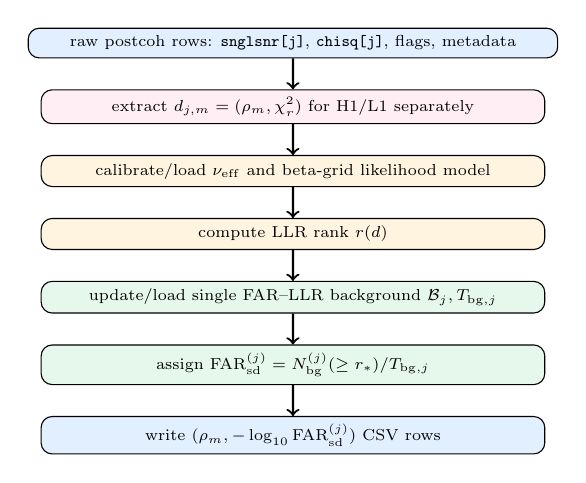
\begin{tikzpicture}[scale=0.82, transform shape, node distance=0.48cm, every node/.style={font=\scriptsize}]
\node[draw, rounded corners, fill=softblue, minimum width=8.2cm] (a) {raw postcoh rows: \code{snglsnr[j]}, \code{chisq[j]}, flags, metadata};
\node[draw, rounded corners, fill=singlebg, below=of a, minimum width=7.8cm] (b) {extract \(d_{j,m}=(\rho_m,\chi_r^2)\) for H1/L1 separately};
\node[draw, rounded corners, fill=softorange, below=of b, minimum width=7.8cm] (c) {calibrate/load \(\nu_{\mathrm{eff}}\) and beta-grid likelihood model};
\node[draw, rounded corners, fill=softorange, below=of c, minimum width=7.8cm] (d) {compute LLR rank \(r(d)\)};
\node[draw, rounded corners, fill=softgreen, below=of d, minimum width=7.8cm] (e) {update/load single FAR--LLR background \(\mathcal B_j,T_{\mathrm{bg},j}\)};
\node[draw, rounded corners, fill=softgreen, below=of e, minimum width=7.8cm] (f) {assign \(\mathrm{FAR}_{\mathrm{sd}}^{(j)}=N_{\mathrm{bg}}^{(j)}(\ge r_*)/T_{\mathrm{bg},j}\)};
\node[draw, rounded corners, fill=softblue, below=of f, minimum width=7.8cm] (g) {write \((\rho_m,-\log_{10}\mathrm{FAR}_{\mathrm{sd}}^{(j)})\) CSV rows};
\foreach \x/\y in {a/b,b/c,c/d,d/e,e/f,f/g}
  \draw[->, thick] (\x) -- (\y);
\end{tikzpicture}
\end{center}
\end{frame}

\begin{frame}{Validation Plan}
\small
The single branch needs validation in increasing order of risk:
\begin{enumerate}
  \item \textbf{Syntax and import checks}: \code{python -m py_compile} for the new Python files; \code{bash -n pipeline.sh}.
  \item \textbf{Unit checks}: central chi-square logpdf, noncentral Poisson-mixture logpdf, beta-mixture normalization, monotonic rank-tail count.
  \item \textbf{Toy rows}: fake postcoh rows with known foreground/background/empty behavior.
  \item \textbf{Small OzSTAR segment}: run \code{bash pipeline.sh --single} on a short known-good frame/cache segment.
  \item \textbf{Cold-start week}: build the first \code{single_far_llr_background.json}.
  \item \textbf{History-file run}: rerun with \code{SINGLE_FAR_BACKGROUND_INPUT} and confirm FAR assignment uses loaded background while appending new ranks/livetime.
\end{enumerate}
\end{frame}

\begin{frame}{Scientific Checks Before Trusting FAR}
\small
\begin{itemize}
  \item Check that the background \(\chi_r^2\) distribution is close enough to the fitted reduced chi-square model in each SNR bin.
  \item Check whether \(\nu_{\mathrm{eff}}\) depends strongly on detector, bank, template duration, or SNR.
  \item Validate \(\beta_{\max}\) and the beta prior with injections; the current uniform prior is a modeling convention.
  \item Verify that H1 and L1 single categories have independent livetime accounting.
  \item Confirm that copied H/L detector-local fields from coexistence rows are not removed from the coherent branch.
  \item Decide how to handle zero exceedance counts: empirical upper limit \(1/T_{\mathrm{bg}}\) or a fitted tail extrapolation.
\end{itemize}
\end{frame}

\begin{frame}{Main Risk: Rank Consistency Across Background Files}
\small
If an old background file contains ranks computed with one likelihood calibration, and the new run changes \(\nu_{\mathrm{eff}}\), beta grid, or SNR weight, then old and new ranks are not directly comparable.

\vspace{0.7em}
The local implementation handles this by storing the likelihood model in the FAR--LLR background JSON.

\vspace{0.7em}
Recommended production policy:
\begin{enumerate}
  \item if \code{SINGLE_FAR_BACKGROUND_INPUT} is used, load its likelihood model and do not recalibrate by default;
  \item if a new calibration is required, rebuild the rank background from raw stored background features or start a new background file version;
  \item store model version and calibration metadata in every background file.
\end{enumerate}
\end{frame}

\begin{frame}{Minimal Completion Sequence}
\small
\begin{enumerate}
  \item Merge main SPIIR and \code{wguo-single-detector} extraction into Eric branch.
  \item Ensure \code{pipeline.sh --single} creates \code{sdpostcoh*.xml.gz} while coherent branch continues.
  \item Install \code{single_detector_far.py} and \code{combine_background_far.py}.
  \item Build/load \code{single_far_llr_background.json}.
  \item Calibrate \(\nu_{\mathrm{eff}}\) from background rows in H1/L1 categories.
  \item Compute LLR rank for all background and foreground single features.
  \item Assign FAR through the rank-tail formula.
  \item Write the single CSV with \(\rho=\code{snglsnr[j]}\) and \(y=-\log_{10}\mathrm{FAR}_{\mathrm{sd}}^{(j)}\).
  \item Later merge with coherent products only after each branch has assigned calibrated FAR.
\end{enumerate}
\end{frame}

\begin{frame}{Final Deliverable of the Single Branch}
\small
The completed single branch should produce rows like:
\[
\begin{array}{cccccc}
\text{category} & \text{detector} & \rho & \chi^2 & r & -\log_{10}\mathrm{FAR} \\
\hline
\mathrm{H1\_sd} & \mathrm{H1} & \code{snglsnr[H1]} & \code{chisq[H1]} & r_{\mathrm{H1}} & -\log_{10}\mathrm{FAR}_{\mathrm{H1}} \\
\mathrm{L1\_sd} & \mathrm{L1} & \code{snglsnr[L1]} & \code{chisq[L1]} & r_{\mathrm{L1}} & -\log_{10}\mathrm{FAR}_{\mathrm{L1}}
\end{array}
\]

\proposal{
This is the correct endpoint for the current study: a calibrated single-detector FAR plane.  The raw feature plane \((\rho_m,\chi_r^2)\) is an intermediate; the final comparable quantity is \((\rho_m,-\log_{10}\mathrm{FAR}_{\mathrm{sd}})\).
}
\end{frame}

\end{document}
